\documentclass{llncs}

   \usepackage{graphicx} %%% TO BE INSERTED %%%

%

%%\begin{document}
\title{URDAD as a Quality Driven Analysis and Design Methodology}
%%\subtitle{Subtitle of your contribution}

%%----Other way of representing the authors----
%%\author	{Riaan Klopper \email{(riaan.klopper2@standardbank.co.za)}\\ 
%%		Fritz Solms\email{(fritz@solms.co.za)}\\
%%		Stefan Gruner \email{(sgruner@cs.up.ac.za)}\\
%%		Derrick Kourie \email{(dkourie@cs.up.ac.za)}}
%%\institute{Department of Computer Science, \\University of Pretoria, South Africa}

\author{Riaan Klopper\inst{1}\email{(riaan.klopper2@standardbank.co.za)} \and Stefan Gruner\inst{1}\email{(sgruner@cs.up.ac.za)}\and Derrick Kourie\inst{1}{(dkourie@cs.up.ac.za)}\and Fritz Solms\inst{2}\email{(fritz@solms.co.za)}}

\institute{Department of Computer Science, University of Pretoria, South Africa,\\
%%\email{riaan.klopper2@standardbank.co.za; sgruner@cs.u.ac.za; dkourie@cs.up.ac.za} -- I moved the email addresses next to the names
\and Solms Training and Consulting, South Africa,\\
%%\email{fritz@solms.co.za}
}

\begin{document}	
\maketitle



%========================================================================================

\section{The URDAD methodology}

URDAD \cite{Solms2007_TechnologyNeutralDesignViaUrdad, Solms2008_GeneratingPimUsingUrdad}
is an analysis and design methodology used for technology neutral design generating
the Platform Independent Model (PIM) of the Model-Driven Architecture. It is currently largely used within the business sector for technology neutral business process design.

The core aims of URDAD are
\begin{itemize}
  \item to make it simpler for experts from the utility domain (e.g.\ business analysts)
		  to perform the technology neutral design leading to the PIM by providing a step
		  for step design process with well defined inputs and outputs for each step (domain
		  experts need not know anything	about the implementation infrastructure,
		  i.e.\ about the architecture and technologies within which the process is to be deployed),
  \item to include quality drivers within the analysis and design methodology ensuring that
		the resultant PIM has certain desired qualities and simplifying the generation of
		quality verification tools, and
  \item to simplify the implementation mapping through a well defined structure for the PIM.
\end{itemize}

URDAD starts with the premise that architecture/infrastructure and design can be viewed as orthogonal with architecture addressing the quality requirements and design addressing the functional requirements. Ultimately the designed process needs to be deployed into some implementation architecture. If, for example, the implementation architecture


\subsection{Analysis and technology-neutral design across levels of granularity}

URDAD envisages that business analysts across the organization collaborate to incrementally build the organization's business model with business analysts from different business domains contributing to different responsibility domains and at different levels of granularity.
For example, business analysts from the claims department of an insurer would define the highe level business process for processing a claim, requiring that one of the services required would be that of assessing to what extend a policy covers a claim. They may not have the business knowledge to know how the claim coverage is to be determined. The business process for the lower level service of assessing the claim coverage could be fed into the PIM by the business analysts of the policies department.

%=================================================

\subsection{URDAD steps}

The steps of the URDAD methodology are shown in the first two swim lanes of
figure \ref{fig:methodology} while the implementation swim lane shows the
standard MDA steps for mapping the PIM onto an implementation. 

\begin{figure}[h]
	\begin{center}
		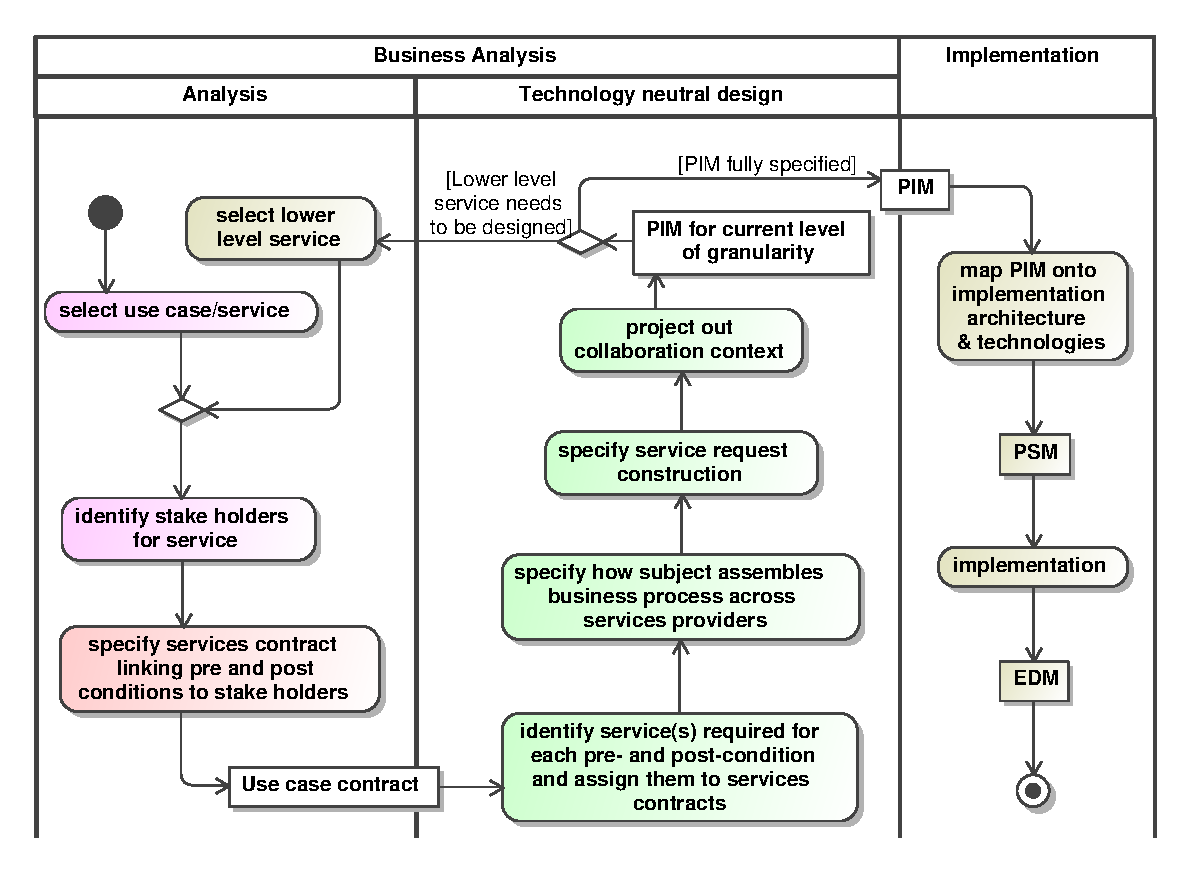
\includegraphics[width=\textwidth]{methodology}
		\caption{The URDAD methodology.}
		\label{fig:methodology}
	\end{center}
\end{figure}

The process is iterative around use cases and incremental across levels of
granularity. Note that for each level of granularity there is both, an analysis
as well as a design phase. The output of the analysis phase is the use
case contract the functional and non-functional requirements for the use
case. The output of the design phase is the PIM for that level of
granularity containing the services contracts for the service providers
required for that level of granularity and the business process assembled
from these services.

On of the services from the current level of granularity is then selected for the use case for the next lower level of granularity and the process is repeated.
The lowest level of granularity is reached if either a particular domain
of responsibility is outsourced, or if the functional requirements need not be
refined any further.

\cite{Solms2007_TechnologyNeutralDesignViaUrdad} provides more details of the URDAD methodology as well as an example of applying the URDAD analysis and design methodology to the business process for processing an insurance claim.

%------------------------------

\subsection{Components of an URDAD based PIM}

In order to contain sufficient information for an implementation mapping onto
some externally defined architecture, 
URDAD generates a PIM containing the following artifacts:
\begin{description}
  \item[Services contracts:] Full services contracts for any service provider required at that level of granularity. These services contracts can be realized by manual or automated work flow steps, external service providers or by processes deployed within off-the shelf solutions.

  \item[Business process specifications] The specification on how a business
	process at any level of granularity is assembled from the services
	defined within the services contracts for that level of granularity.	

  \item[Request construction] The PIM must contain the specification on
	how the information required for a service request is assembled
	from the currently available information.

  \item[Data structure specification] The model must contain the data structure
	requirements in a technology neutral way.
\end{description}


%==============================================================================================

\begin{thebibliography}{10}

\bibitem{Arthur1991_FrameworkForAssessingMethodologies}
J. D. Arthur and R.~E. Nance
\newblock A Framework for Assessing the Adequacy and Effectiveness of Software Development Methodologies
\newblock Technical report TR 91-28, Department of Computer Science, Virginia Polytechnic Institute and State University, 1991

\bibitem{Solms2007_TechnologyNeutralDesignViaUrdad}
F. Solms.
\newblock Technology neutral business process design using {URDAD}.
\newblock In H.~Fujita and D.~Pisanelli, editors, {\em New Trends in Software
  Methodologies, Tools and Techniques}, Frontiers in Artificial Intelligence
  and Applications, pages 52--70. IOS Press, 2007.

\bibitem{Solms2008_GeneratingPimUsingUrdad}
F. Solms and D. Loubser.
\newblock Generating MDA's Platform Independent Model using {URDAD}.
\newblock Submitted for publication.

\bibitem{martin:agileSoftwareDevelopment}
R.~C. Martin.
\newblock {\em Agile Software Development, Principles, Patterns, and
  Practices}.
\newblock Prentice-Hall, 2002.

\end{thebibliography}


\end{document}



\bibitem{aizenbud-reshef:modelTraceability}
N.~Aizenbud-Reshef, J.~R. Brian T.~Nolan, and Y.~Shaham-Garifi.
\newblock Model traceability.
\newblock {\em IBM Systems Journal}, 45(3):515--526, 2006.

\bibitem{artus:soaRealization}
D.~J. Artus.
\newblock Soa realization: Service design principles.
\newblock Technical report, IBM, February 2006.

\bibitem{Bass:softwareArchitecture}
L.~Bass, P.~Clements, and R.~Kazman.
\newblock {\em Software Architecture in Practice, Second Edition}.
\newblock Addison-Wesley Professional, April 2003.

\bibitem{berard:whatIsMethodology}
E.~V. Berard.
\newblock What is a methodology?
\newblock White paper, The Object Agency, 1995.

\bibitem{sun:javaee}
S.~Corporation.
\newblock Java ee at a glance.
\newblock http://java.sun.com/javaee/.

\bibitem{demarco:structuredAnalysis}
T.~DeMarco.
\newblock {\em Structured Analysis and System Specification}.
\newblock Yourdon Press, 1979.

\bibitem{dick:designTraceability}
J.~Dick.
\newblock Design traceability.
\newblock {\em IEEE Software}, 22(6):14--16, November 2005.

\bibitem{erl:soa}
T.~Erl.
\newblock {\em Service-Oriented Architecture (SOA): Concepts, Technology, and
  Design}.
\newblock Prentice Hall PTRs, August 2005.

\bibitem{frankel:enterpriseMDA}
D.~S. Frankel.
\newblock {\em Model Driven Architecture: Applying MDA to enterprise
  computing}.
\newblock John Wiley \& Sons, New York, 2003.

\bibitem{kruchten:rup}
P.~Kruchten.
\newblock {\em The Rational Unified Process}.
\newblock Addison Wesley, 2000.

\bibitem{lenz:softwareReuse}
M.~Lenz, H.~A. Schmid, and P.~F. Wolf.
\newblock Software reuse through building-blocks.
\newblock {\em IEEE Software}, 4(4):32--42, 1987.

\bibitem{rosenberg:useCaseDrivenObjectModeling}
D.~Rosenberg and K.~Scott.
\newblock {\em Use Case Driven Object Modeling with UML: A Practical Approach}.
\newblock Addison-Wesley Professional, New York, 1999.

\bibitem{rumbaugh:umlReference}
J.~Runbaugh, I.~Jacobson, and G.~Booch.
\newblock {\em Unified Modeling Language Reference Manual, 2nd Edition}.
\newblock Addison-Wesley Professional, July 2004.

\bibitem{schmidt:modelDrivenEngineering}
D.~C. Schmidt.
\newblock Model driven engineering.
\newblock {\em IEEE Computer}, 39(2):25--31, February 2006.

\bibitem{selic:pragmaticsOfModelDrivenDevelopment}
B.~Selic.
\newblock The pragmatics of model driven development.
\newblock {\em IEEE Software}, 20(5):19--25, September/October 2003.

\bibitem{siegel:developingInMDA}
J.~Siegel.
\newblock Developing in omg's model-driven architecture.
\newblock White paper, Object Management Group, November 2001.

\bibitem{voas:softwareTestability}
J.~M. Voas and K.~W. Miller.
\newblock Software testability: The new verification.
\newblock {\em IEEE Software}, 12(3):17--28, MAY 1995.

\bibitem{wirfs-brock:designSimplicity}
R.~J. Wirfs-Brock.
\newblock Toward design simplicity.
\newblock {\em IEEE Software}, 24(2):9--11, March/April 2007.

\bibitem{wirfs-brock:objectDesign}
R.~J. Wirfs-Brock and A.~McKean.
\newblock {\em Object Design: Roles, Responsibilities and Collaboration}.
\newblock Addison-Wesley Professional, New York, 2002.

\bibitem{wirfs-brock:responsibilityDrivenApproach}
R.~J. Wirfs-Brock and B.~Wilkerson.
\newblock Object-oriented design: A responsibility-driven approach.
\newblock In {\em OOPSLA '89 Proceedings}, pages 71--75. TeX Users Group,
  October 1989.
